\documentclass{standalone}

\usepackage[OT1]{fontenc}
\renewcommand*\familydefault{\sfdefault}
\usepackage{helvet,sfmath}
\usepackage{siunitx}

\usepackage{tikz}
\usetikzlibrary{arrows,calc,patterns}
\usepackage{tikz,tkz-euclide}
\usepackage{circuitikz}

%% Color %%
\definecolor{BlueDefault}{rgb}{0.2,0.2,0.7}
\definecolor{Fr4}{RGB}{228, 188, 65}
\definecolor{Copper}{RGB}{184, 115, 51}

\begin{document}

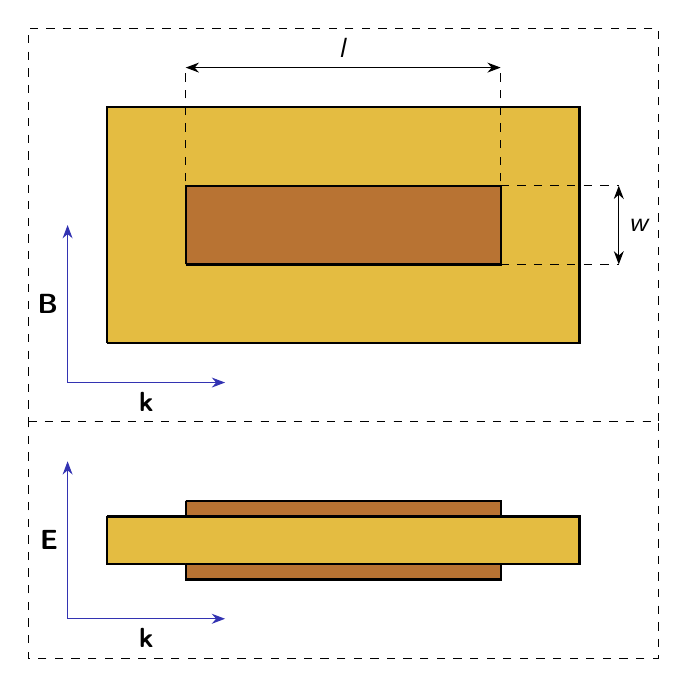
\begin{tikzpicture}[scale=1]
    %%CWP in BK plane
    \draw[fill=Fr4, thick] (-3,0) to (3,0) to (3,3) to (-3,3) to (-3,0);
    \draw[fill=Copper, thick] (-2,1) to (2,1) to (2,2) to (-2,2) to (-2,1);
    %%Parameters
    \draw[dashed] 
    (2,1) to (2,3.5)
    (-2,1) to (-2,3.5)
    (2,1) to (3.5,1)
    (2,2) to (3.5,2)
    ;
    \draw[Stealth-Stealth] (2,3.5) to (-2,3.5);
    \draw[Stealth-Stealth] (3.5,1) to (3.5,2);
    \draw
    (3.5,1.5) node[right]{\(w\)}
    (0,3.5) node[above]{\(l\)}
    ;
    %% EM fields
    \draw[BlueDefault, -Stealth] (-3.5,-0.5) to (-3.5,1.5);
    \draw[BlueDefault, -Stealth] (-3.5,-0.5) to (-1.5,-0.5);
    \draw
    (-3.5,0.5) node[left]{\(\mathbf{B}\)}
    (-2.5,-0.5) node[below]{\(\mathbf{k}\)}
    ;
    \draw[dashed] (-4,-1) to (4,-1) to (4,4) to (-4,4) to (-4,-1);
    %%%%%%%%%%%%%%%%%%%%%%%%%%%%%%%%%%%%%%%%%%%%%%%%

    %%Structure in EK plane
    \draw[fill=Fr4, thick] (-3,-2.2) to (3,-2.2) to (3,-2.8) to (-3,-2.8) to (-3,-2.2);
    \draw[fill=Copper, thick] 
    (-2,-2) to (2,-2) to (2,-2.2) to (-2,-2.2) to (-2,-2)
    (-2,-2.8) to (2,-2.8) to (2,-3) to (-2,-3) to (-2,-2.8)
    ;
    %% EM fields
    \draw[BlueDefault, -Stealth] (-3.5,-3.5) to (-3.5,-1.5);
    \draw[BlueDefault, -Stealth] (-3.5,-3.5) to (-1.5,-3.5);
    \draw
    (-3.5,-2.5) node[left]{\(\mathbf{E}\)}
    (-2.5,-3.5) node[below]{\(\mathbf{k}\)}
    ;
    \draw[dashed] (-4,-1) to (4,-1) to (4,-4) to (-4,-4) to (-4,-1);
    
\end{tikzpicture}

\end{document}

